%!TEX root=../paper.tex

\chapter{GreenWeb: Web Language Extensions for Energy-Efficient Web Computing}
\label{sec:lang}

%Web application developers today must be conscious of energy efficiency. Current abstractions between software and hardware, however, do not provide developers opportunities to optimize for energy efficiency. Instead, energy optimizations are mostly conducted at the hardware and OS level via techniques such as dynamic voltage and frequency scaling. Although effective from a hardware perspective, the key limitation of these techniques is that they are not aware of user quality-of-service (QoS) expectation and may lead to poor experience~\cite{big-little, ebs, pgdvfs}. Failing to deliver desirable QoS experience can cause severe consequences. For example, a 1-second delay in webpage load time costs Amazon \$1.6 billion annual lost in sales~\cite{Eaton:2013uq}.

Web languages are at the interface between applications and Web runtime. Traditionally, Web developers use Web languages to express structure, style, and functionality of an application while relying on the underlying system to perform energy optimizations without compromising user QoS experience. However, as mobile users become increasingly aware of poor energy behavior of applications~\cite{badappreviews,appdeletion}, Web developers today must be  explicitly conscious of energy efficiency. Current programming language abstractions, however, provide developers few opportunities to optimize for energy efficiency. Instead, energy optimizations are mostly conducted at the hardware and OS level via techniques such as dynamic voltage and frequency scaling. Although effective from a system perspective, the key limitation of these techniques is that they are not aware of user quality-of-service (QoS) expectations and may lead to poor experience~\cite{big-little,ebs,pgdvfs}. Failing to deliver a desirable QoS experience can cause severe consequences. For example, a 1-second delay in webpage load time costs Amazon \$1.6 billion annual sales lost~\cite{Eaton:2013uq}.

In this chapter, I present \greenweb, a set of Web language extensions defined as Cascading Style Sheet (CSS) rules that allow Web developers to express user QoS expectation at an abstract level. Based on the programmer-guided QoS information, the runtime substrate of \greenweb could then dynamically determine how to deliver the target QoS experience while minimizing the energy consumption.

To help Web developers reason about QoS constraints in Web applications, our \textit{key insight} is that user QoS experience can be sufficiently captured by two fundamental abstractions: \textit{QoS type} and \textit{QoS target}. Intuitively, QoS type characterizes whether users perceive QoS experience by interaction responsiveness or animation smoothness, and QoS target denotes the performance level that is required to deliver a desirable user experience for a specific QoS type. \greenweb provides specific language constructs for expressing the two QoS abstractions and thus empowering Web developers to provide ``hints'' to guide energy optimizations.

Allowing programmers to annotate QoS information in applications is both \textit{precise} and \textit{efficient}. It is precise because only developers have the exact knowledge of code logic. They can provide QoS type and target information that is difficult for the runtime to infer. It is efficient because it does not entail performance and energy overhead of runtime detection. Such a design philosophy is similar to traditional pragma-based programming APIs such as OpenMP. For example, the ``\texttt{omp for}'' pragma in OpenMP indicates that iterations in a \texttt{for} loop are completely independent such that the runtime can safely parallelize the loop without the need to check for correctness. Similarly, \greenweb annotations would allow the Web runtime to perform ``best-effort'' optimizations without having to infer QoS information.

The rest of this chapter is organized as follows. \Sect{sec:lang:eqos} discusses the relationship between QoS, performance, and energy consumption. It lays the foundation of abstracting user QoS experience. \Sect{sec:lang:abst} defines two abstractions that are critical to mobile user QoS experience, and \Sect{sec:lang:spec} describes the proposed \greenweb language constructs that express the two abstractions. \Sect{sec:lang:auto} presents \autogreen to demonstrate the feasibility of automatically applying \greenweb annotations to a Web application. \Sect{sec:lang:inter} discusses the relationship between the \greenweb extensions and the \webrt runtime, and argue that \greenweb and \webrt are synergistic while independent. \Sect{sec:lang:disc} discusses the implications and limitations of the current design and implementation of \greenweb. Finally, \Sect{sec:lang:related} puts \greenweb in the general context of language support for performance and energy-efficiency.

\section{Trade-off Between QoS, Performance, and Energy}
\label{sec:lang:eqos}

We illustrate the relationship between application QoS, performance, and energy savings in~\Fig{fig:eqos}. Performance degrades from left to right on the~\textit{x}-axis. The left and right~\textit{y}-axes indicate QoS and energy savings, respectively. Foundational work in human-computer interaction research~\cite{eventlatency,designUI,info_vis,response_time,percent_done,usability_engineering} indicates that interactive application QoS can be classified into three distinct states as machine performance degrades: \textit{imperceptible} $[P_H,P_I]$, \textit{tolerable} $(P_I,P_U]$, and \textit{unusable} $(P_U,P_L]$.

\begin{figure}[t]
\centering
\captionsetup{width=.9\columnwidth}
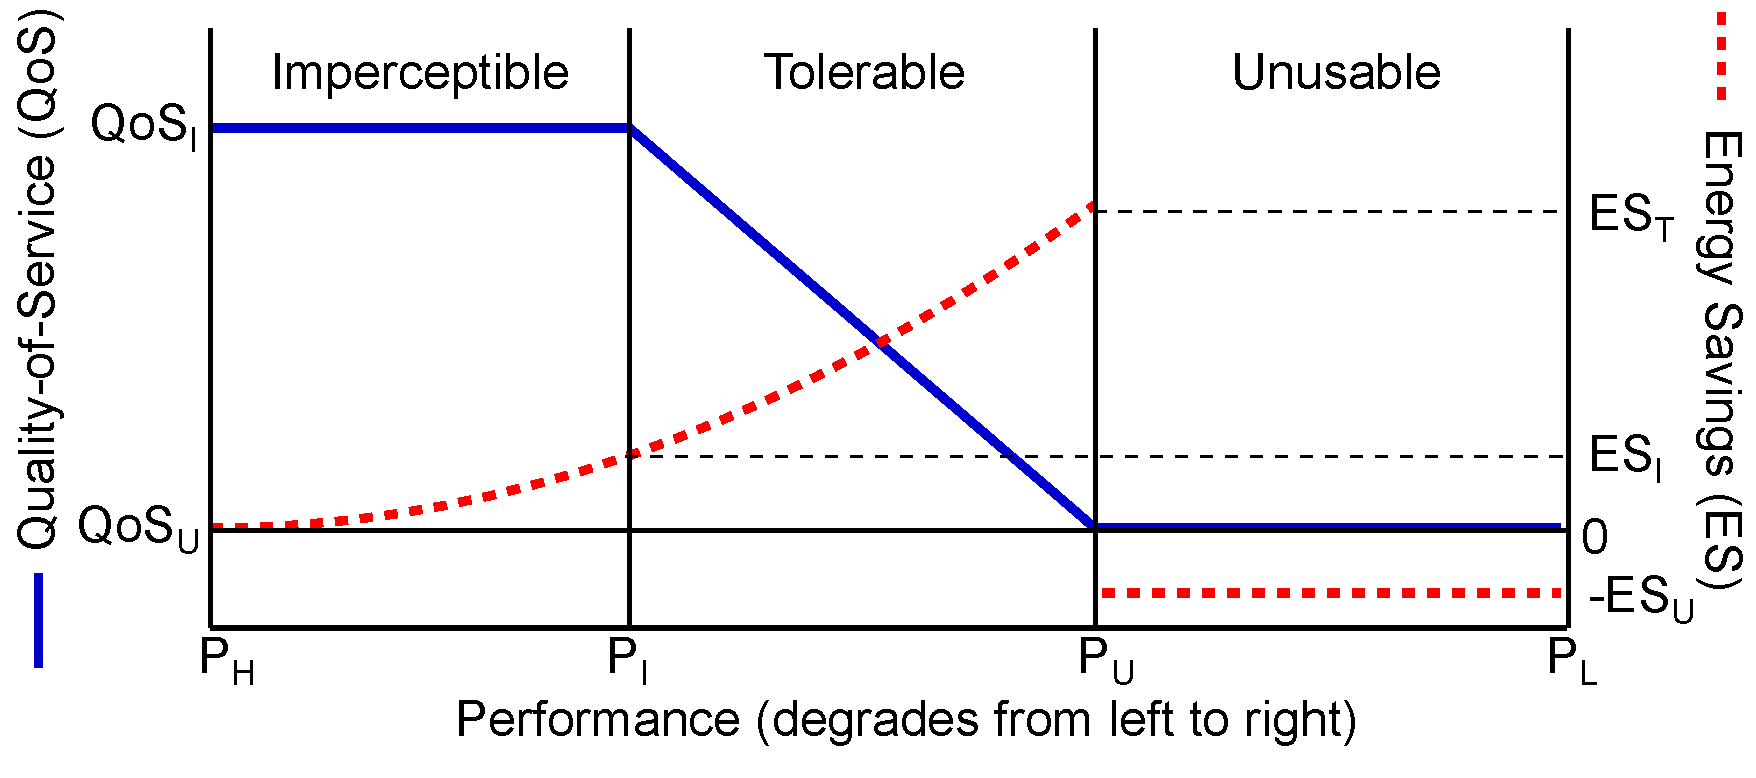
\includegraphics[trim=0 0 0 0, clip, width=.9\columnwidth]{eqos}
\caption{The interplay between QoS, performance, and energy.}
\label{fig:eqos}
\end{figure}

In the imperceptible region, performance can degrade without any user-perceptible QoS loss while achieving more energy savings. Imperceptible QoS, $QoS_I$, is maintained until performance reaches $P_I$, the lowest performance level that provides $QoS_I$. In the imperceptible region, supplying higher performance simply leads to more energy waste without adding any end-user value. For example, the most conservative approach to guarantee application QoS is to supply the peak performance of $P_H$; it leads to an energy waste of $ES_I$. Beyond $P_I$, application QoS enters the tolerable region, where QoS deteriorates as performance reduces, but still remains tolerable. Any QoS could be acceptable in this region depending on the usage scenario or specific user pattern~\cite{usagepattern,satscore}. Therefore, the tolerable QoS region exhibits a traditional performance-energy trade-off space. As performance further degrades, QoS is eventually violated at $P_U$, which is the performance limit where users no longer feel engaged by the application. At $P_U$ and beyond, users abandon the service. As a result, any energy consumed up until the service abandonment ($ES_U$) is wasted, because the underlying computation does not provide any utility to the user.

In summary, QoS-aware energy-efficiency optimization implies one of the following two optimization strategies depending on user QoS expectation. First, when the QoS expectation is high, guarantee imperceptible QoS experience with the minimal energy by exploiting the performance slack between $P_H$ and $P_I$. Second, when the user QoS expectation is low, guarantee usable QoS experience with the minimal energy by achieving a performance of $P_U$.

\section{QoS Abstractions for Web Applications}
\label{sec:lang:abst}

Expressing user QoS experience to the underlying system is the key in QoS-aware energy efficiency optimizations. However, today's Web languages do not allow expressing QoS information. Programmers need new \textit{abstractions}. We propose two abstractions, QoS type and QoS target, that capture two fundamental aspects of user QoS experience in Web applications. Such QoS abstractions hide the complexity of the specific application implementation from underlying systems while still providing enough details to guide energy optimizations. This section introduces the abstractions, and the next section~(\Sect{sec:lang:spec}) describes the proposed language constructs that enable programmers to express the abstractions.

Abstracting user QoS experience requires us to first understand how users assess QoS experience in mobile Web applications. To that end, we leverage the LTM user-application interaction model described in \Sect{sec:runtime:overview}. The LTM model captures three fundamental user interactions in mobile Web applications (Loading-Tapping-Moving) and gives us a framework for reasoning about user QoS experience. Based on the LTM model, we propose the QoS type~(\Sect{sec:lang:abst:type}) and QoS target~(\Sect{sec:lang:abst:target}) abstractions. We discuss why they are necessary and sufficient to express QoS information for QoS-aware energy efficiency optimizations.

\subsection{QoS Type}
\label{sec:lang:abst:type}

We define an abstraction called \textit{QoS type} to capture different ways that users interpret the QoS experience. Two major QoS types exist: \textit{single} and \textit{continuous}. Intuitively, they indicate whether the QoS experience is determined by the ``responsiveness'' of a single frame or the ``smoothness'' of a continuous sequence of frames, respectively. Let us use the LTM model to elaborate on the two QoS types.

%!TEX root=../../paper.tex

\begin{table}[t]
\large
\centering
\caption{Interactions in mobile Web applications fall into three categories based on different QoS type and QoS target combinations.}
\renewcommand*{\arraystretch}{1.2}
\renewcommand*{\tabcolsep}{10pt}
\resizebox{\columnwidth}{!}
{
  \begin{tabular}{l l l c}
  \toprule[0.15em]
  \bigstrut\textbf{QoS Type} & \bigstrut\textbf{\specialcell{QoS Target\\($P_I$, $P_U$)}} & \multicolumn{1}{c}{\bigstrut\textbf{~~~~~~~~Description}} & \bigstrut\textbf{Interaction}\\
  \midrule[0.05em]
  Continuous & (16.6, 33.3) ms & \specialcell{QoS experience is evaluated\\by \textit{continuous} frame latencies.} & T, M\\
  \midrule
  \multirow{2}{*}[-23pt]{Single} & (100, 300) ms & \specialcell{QoS experience is evaluated
\\by \textit{single} frame latency. Users
\\expect \textit{short} response period.} & T \\ \cline{2-4}
  & (1, 10) s & \specialcell{QoS experience is evaluated
\\by \textit{single} frame latency. Users
\\expect \textit{long} response period.} & L, T \\
  \bottomrule[0.15em]
  \end{tabular}
}
\label{tab:qos_info}
\end{table}



\paragraph{Single} Some user interactions produce only a single frame, which we call the response frame. The QoS type of these interactions is ``single,'' indicating that user QoS experience is determined by the latency at which the response frame is perceived by users~\cite{eventlatency}. For instance, imagine a fingertap interaction (T) that opens a search box in a Web application. Users perceive the effect of the fingertap when the application displays a response frame---the frame with the search box displayed. Web application loading process (L) also falls in this category. This is because although there are several intermediate frames being produced during the loading process, user QoS experience is largely determined by the latency of the ``first meaningful frame''~\cite{fmf}, which indicates that a Web application is usable by users.

Under the ``single'' QoS type, an ideal energy-efficient system would allocate just enough energy to produce the single response frame and conserve energy afterwards. It is worth noting that the system might not be completely idle after the response frame is delivered. The system could still perform work such as updating the browser cache, performing garbage collection, or rasterizing off-screen pixels. Such ``post-frame'' work is not critical to user QoS experience and could be executed in a low-power mode.

\paragraph{Continuous} The other QoS type is ``continuous,'' corresponding to interactions whose responses are not one single frame but a sequence of continuous frames. User QoS experience is determined by the latency of \textit{each} frame in the sequence rather than one specific frame as in the ``single'' case. Ideally, an energy-efficient Web runtime would allocate just enough energy for each frame in the sequence and conserve energy after all the frames are produced.
%Determining the exact sequence of frames given an input event is a non-trivial task and we discuss it in \Sect{sec:runtime:frame}.

Continuous frames are often found in the form of animations. The simplest form of animation is triggered by finger moving (M) such as scrolling. Tapping (T) can also cause a sequence of frames to be generated. For instance, many Web applications provide a navigation button that dynamically expands when tapped and generates an animation. More complex animations in Web applications can be controlled by \texttt{requestAnimationFrame} (\texttt{rAF}) APIs~\cite{animationtiming} and CSS animation/transition~\cite{cssanimations,csstransitions}.

Distinguishing between ``continuous'' and ``single'' is important. If an event callback triggers an animation but the runtime treats its QoS type as ``single'', the runtime would optimize for only the first frame in the sequence, and thus mis-operates for the remaining frames. On the other hand, if an event produces only a single frame followed by some ``post-frame'' work, a runtime (mistakenly) optimizing for ``continuous'' frame latency would force the hardware to run at the peak performance to execute the ``post-frame'' work (with the intention of generating more frames), leading to energy waste. Whether an event triggers a single frame or a sequence of frames can not be determined a priori. In \Sect{sec:lang} we will introduce a set of language extensions that let developers explicit specify an event's QoS type, through which the runtime could be better informed in optimizations.

\subsection{QoS Target}
\label{sec:lang:abst:target}

Another critical QoS abstraction is \textit{QoS target}, denoting the performance level needed to deliver a certain QoS experience. We use frame latency as a natural choice for the performance metric because frame updates dictate QoS experience. Specifically, we define frame latency as the delay from when an event is initiated by a user to when its corresponding frame(s) show on the display.

Two different QoS targets exist that are critical to user experience: imperceptible target ($P_I$) and usable target ($P_U$)~\cite{ebs}. Imperceptible target delivers a latency that is imperceptible/instantaneous to users. Achieving a performance higher than $P_I$ does not add user perceptible value while unnecessarily wasting energy. The usable target, in contrast, corresponds to a latency that can barely keep users engaged. Delivering a performance lower than $P_U$ may cause users to deem an application unusable and even abandon it.

\paragraph{Single} For interactions with the ``single'' QoS type, QoS target depends on the complexity of the interaction~\cite{eventlatency}. For interactions that are expected to finish quickly, user latency tolerance is low. For instance, a fingertap that displays a search box falls into this category, because displaying a search box is inherently expected to finish ``instantly.'' For these ``lightweight'' interactions, users feel the system is responding instantly at 100~ms, and start thinking that the system is not working after 300~ms~\cite{humanperception}. Thus, 100~ms and 300~ms can be used as the $P_I$ and $P_U$ values, respectively.

In contrast, when users are aware of a computationally intensive job being processed, they tend to have high tolerance for latencies~\cite{usability_engineering}. Psychological study shows that users can subconsciously wait up to 1 second for a job to complete while still staying focused on the current train of thought. Once a job execution exceeds 10 seconds, user attentions are distracted and cannot tolerate the delay~\cite{info_vis,response_time}. Therefore, 1 second and 10 seconds can be treated as the $P_I$ and $P_U$ values for ``heavyweight'' interactions, respectively.

\paragraph{Continuous} For interactions with a ``continuous'' QoS type, 60 and 30 frames per second (FPS) deliver a ``seamless'' and ``just playable'' user experience, respectively~\cite{fps_target}. Thus, a performance level that guarantees 16.6~ms and 33.3~ms frame latency can be regarded as the imperceptible and usable QoS target, respectively. It is worth noting that the QoS target applies to each frame rather than an average latency. This is because human eyes are very sensitive to frame variance. Tiny hitches in a high volume of frames can cause a poor QoS experience and even headaches~\cite{jankbusting,adaptivevsync}.

User interactions fall into three distinct categories based on the different QoS type and QoS target combinations as listed in \Tbl{tab:qos_info}. Although the absolute values of QoS target ($P_I$ and $P_U$) in each category can vary slightly with user perceptibility, their magnitudes differ significantly across categories (i.e., tens of milliseconds versus hundreds of milliseconds versus seconds). Thus, QoS target is an important abstraction to differentiate different performance requirements.

\section{QoS-Aware Web API Design}
\label{sec:lang:spec}

We now present \greenweb, a set of Web language extensions that lets application developers easily express the two QoS abstractions as program annotations. We first discuss the design principles of \greenweb extensions (\Sect{sec:lang:spec:principles}). We then describe the design and specification of \greenweb~(\Sect{sec:lang:spec:api}). We then present usage scenarios to demonstrate the expressiveness and modularity of the \greenweb design~(\Sect{sec:lang:spec:ex}).

\subsection{Design Principles}
\label{sec:lang:spec:principles}

\greenweb extensions follow three design principles. First, adding or removing \greenweb annotations does not change application functionality and correctness. In other words, \greenweb annotations are \textit{modular} components in an application. Modularity allows developers who are unfamiliar with application logic to still be able to express QoS information, and allows removing problematic annotations in a non-interference manner.

Second, \greenweb is \textit{intuitive} for Web application developers to use in that it does not require developers to specify absolute values of QoS targets (although this option is provided if needed). This is important because developers may not have quantitative knowledge about user perceptibility. Instead, developers provide a qualitative specification. This design makes the APIs more expressive, and provides flexibility for runtime implementation. 

Third, \greenweb syntax is \textit{compatible} with current Web language specifications, which is crucial for lowering the learning curve and ensuring programmer productivity.

\subsection{QoS-Aware Web API Design}
\label{sec:lang:spec:api}

% !TEX root = ../../paper.tex

\begin{table}[p]
\large
\centering
\caption{Specifications of the \greenweb APIs. Each API is a new CSS rule specifying the QoS information when a particular event is triggered on certain Web application element.}
\renewcommand*{\arraystretch}{1.1}
\renewcommand*{\tabcolsep}{8pt}
\resizebox{\columnwidth}{!}
{
    \begin{tabular}{l l}
    \toprule[0.15em]
    \bigstrut\textbf{Syntax} & \bigstrut\textbf{Semantics} \\
    \midrule[0.05em]
    \specialcell{\texttt{\textcolor{blue}{E:QoS} \{}
\\~~~~\texttt{\textcolor{Green}{onevent-qos:} continuous}
\\\texttt{\}}} & \specialcell{As soon as \texttt{onevent} is triggered on\\DOM element \texttt{E}, the application must\\continuously optimize for frame latency.\\Use the $P_I$ and $P_U$ values in \Tbl{tab:qos_info} as\\the default QoS target for all frames.}\\
    \midrule[0.05em]
    \specialcell{\texttt{\textcolor{blue}{E:QoS} \{}
\\~~~~\texttt{\textcolor{Green}{onevent-qos:} single,}
\\~~~~\texttt{~~~~~~~~~~~~~~short|}
\\~~~~\texttt{~~~~~~~~~~~~~~~long}
\\\texttt{\}}} & \specialcell{Once \texttt{onevent} is triggered on element\\\texttt{E}, the application must optimize for the\\latency of the single frame caused by\\ \texttt{onevent}. Users expext short (long)\\latency. Use the $P_I$ and $P_U$ values in\\\Tbl{tab:qos_info} as the default QoS target.}\\
    \midrule[0.05em]
    \specialcell{\texttt{\textcolor{blue}{E:QoS} \{}
\\~~~~\texttt{\textcolor{Green}{onevent-qos:} continuous|}
\\~~~~\texttt{~~~~~~~~~~~~~~~~~single,}
\\~~~~\texttt{~~~~~~~~~~~~~~~ti-value,}
\\~~~~\texttt{~~~~~~~~~~~~~~~tu-value}

\\\texttt{\}}} & \specialcell{Explicitly specify $P_I$ (\texttt{ti-value}) and\\$P_U$ values (\texttt{tu-value}) for QoS targets.\\Note that both values must either appear\\or be ommitted together.}\\
    \bottomrule[0.15em]
    \end{tabular}
}
\label{tab:api_spec}
\end{table}


\begin{figure}[t]
  \centering
  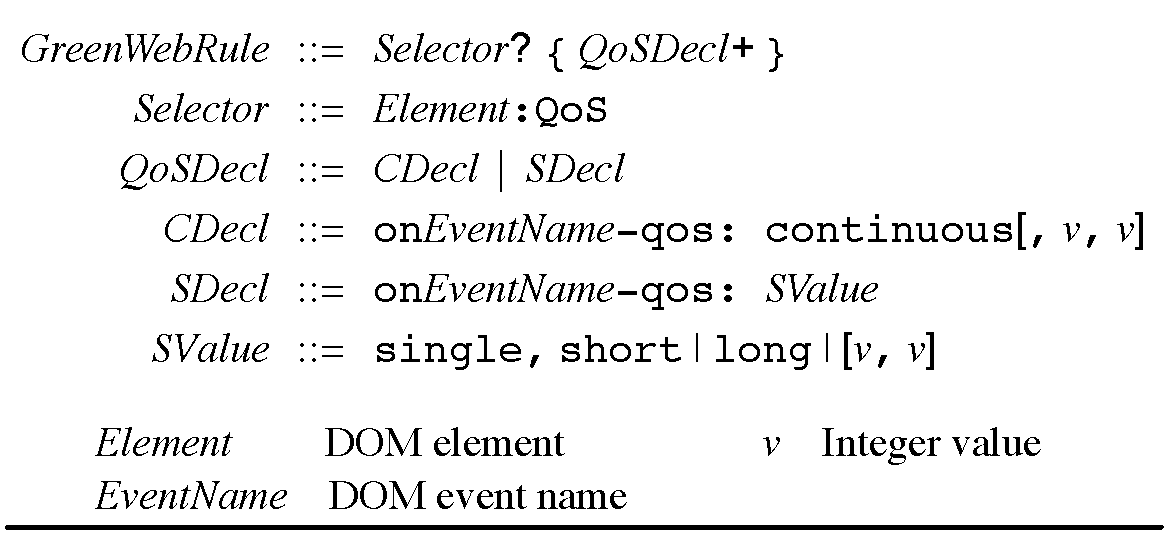
\includegraphics[trim=0 0 0 0, clip, width=.8\columnwidth]{syntax}
  \caption{The syntax of \greenweb language extensions.}
  \label{fig:syntax}
\end{figure}

The \greenweb APIs extend the current CSS language to specify QoS type and QoS target information. We choose CSS because its syntax and semantics naturally allow us to select DOM elements and specify various characteristics. The core of CSS is a set of \textit{style rules}. Each style rule selects specific Web application elements and sets their style properties. A style rule expresses such semantics through two language constructs: a \textit{selector}, which selects specific Web application elements, and a set of style \textit{declarations}, which are $\langle property, value \rangle$ pairs that assign $value$ to $property$. As an example, the following CSS rule \texttt{h1 \{font-weight: bold\}} selects all the \texttt{h1} elements and sets their \texttt{font-weight} property to \texttt{bold}.

Traditionally, CSS supports purely visual style properties such as fonts and colors. Recent development of CSS (e.g., CSS3) lets developers express richer information such as controlling animations~\cite{cssanimations} and adapting to different device form factors~\cite{css3mediaquery}. \greenweb follows this spirit of CSS language evolution and further expands the CSS semantics scope to allow expressing user QoS related information.

\Fig{fig:syntax} shows the \greenweb syntax, and \Tbl{tab:api_spec} lists the semantics of each API. Intuitively, each \greenweb API selects an application element \texttt{E}, and declares CSS properties to express the QoS type and QoS target information when an event \texttt{onevent} is triggered on \texttt{E}. We now describe the details of the \greenweb extensions.

\paragraph{Selector} To decorate a CSS rule as specifying the QoS information of an element, we define a new CSS pseudo-class selector~\cite{css_pseudo_class} ``\texttt{:QoS}.'' An element \texttt{E} is selected using existing selectors, such as ID (\texttt{\#id}) and Class (\texttt{.class}) selectors, before applying the \texttt{:QoS} pseudo-class qualifier. For example, \texttt{div\#intro:QoS} selects the \texttt{div} element with the ID \texttt{intro} before declaring QoS information.

\paragraph{Property} QoS information is expressed as CSS properties in \greenweb. We define a new CSS property called \texttt{onevent-qos}, in which \texttt{onevent} is a DOM event that \greenweb supports. In its simplest form, \texttt{onevent-qos} could be set to \texttt{continuous} (first rule in \Tbl{tab:api_spec}). The semantics of declaring \texttt{onevent-qos: continuous} is that as soon as \texttt{onevent} is triggered on element \texttt{E}, the Web browser runtime must continuously optimize for frame latency until the last relevant frame is generated.

To express the ``single'' QoS type, the \texttt{onevent-qos} property accepts a list of two values separated by a comma, one to indicate that the QoS type is single, and the other to indicate whether users expect a short or long execution period (second rule in \Tbl{tab:api_spec}). For instance, the declaration \texttt{onevent-qos: single, short} expresses that the runtime must optimize for the latency of the single frame caused by \texttt{onevent}, and users expect short frame latency.

Developers do not have to specify the QoS target values; the \greenweb runtime will use the $P_I$ and $P_U$ values in \Tbl{tab:qos_info} as the default QoS target. However, we also provide the flexibility for developers to overwrite the default QoS targets. This is achieved by specifying absolute values of $P_I$ and $P_U$ (in milliseconds) after \texttt{single} or \texttt{continuous}, as shown in the third rule in \Tbl{tab:api_spec}.

\subsection{Example Usage}
\label{sec:lang:spec:ex}

The proposed QoS-aware \greenweb APIs support a wide range of Web application interaction patterns. We explore different usages using two examples.

\begin{figure}[t]
  \centering
  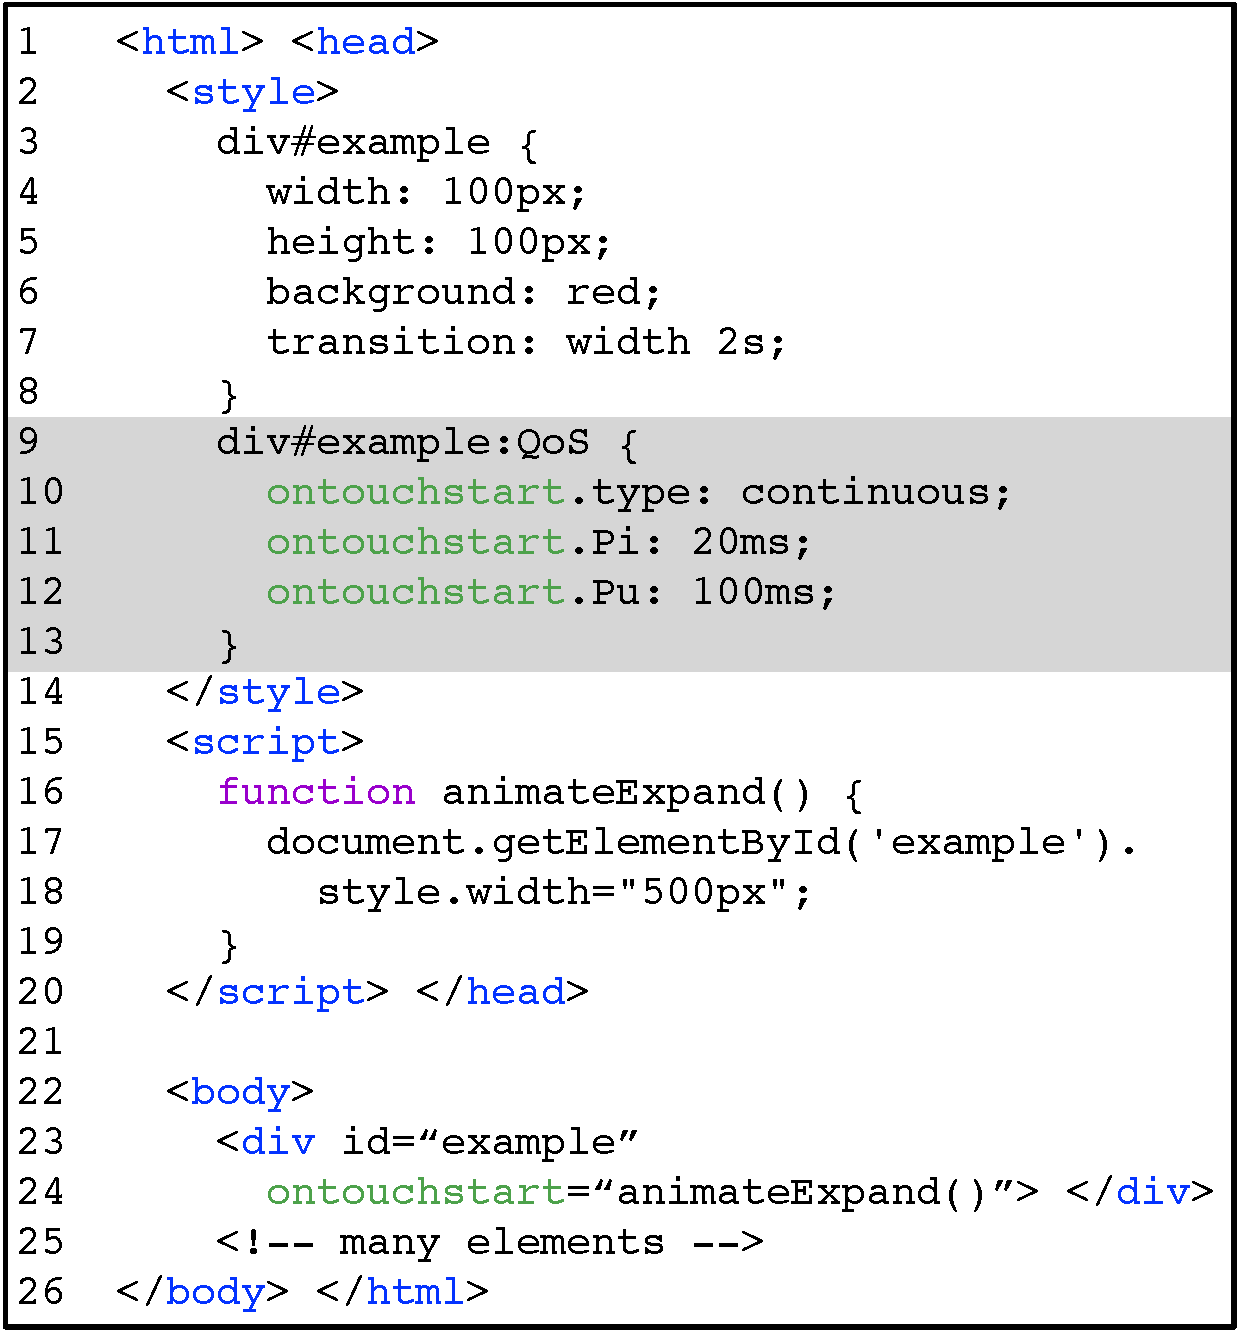
\includegraphics[trim=0 0 0 0, clip, width=.9\columnwidth]{csstransition}
  \caption{Express the QoS type of \texttt{ontouchstart} event as ``continuous,'' and use the default $P_I$ and $P_U$ values.}
  \label{fig:csstransition}
\end{figure}

\begin{figure}[t]
  \centering
  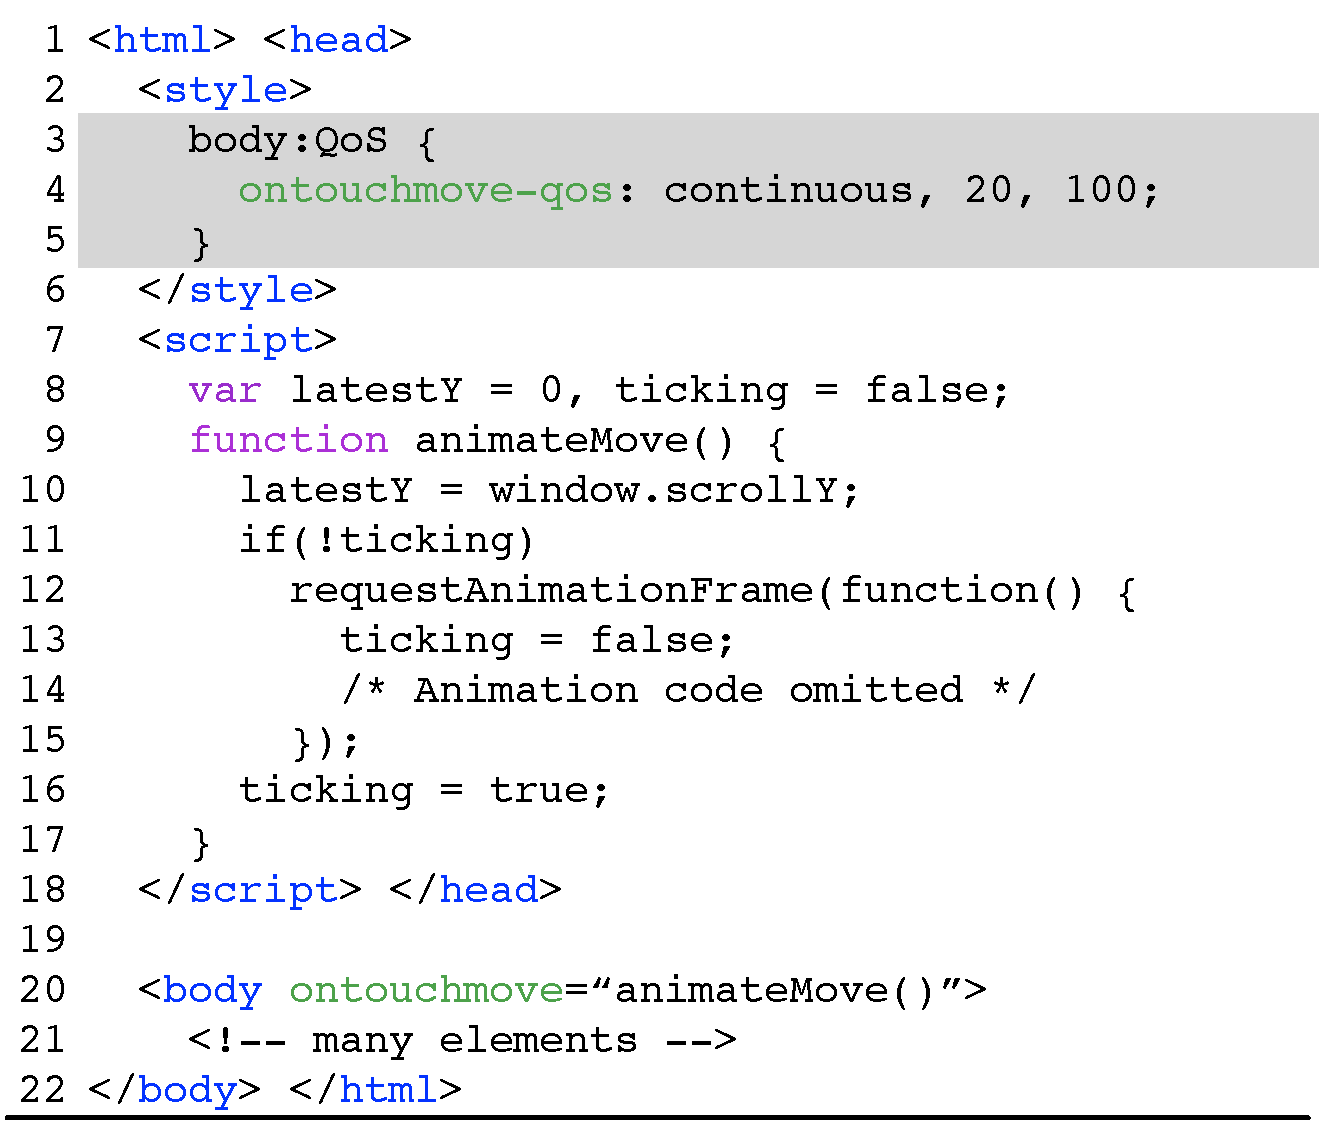
\includegraphics[trim=0 0 0 0, clip, width=.9\columnwidth]{raf}
  \caption{Express the QoS type of \texttt{ontouchmove} event as ``continuous,'' and use 20~ms and 100~ms as the new QoS targets.}
  \label{fig:raf}
\end{figure}

\paragraph{Animations via CSS Transition} The first example involves annotating events that achieve animation using a CSS transition. A CSS transition lets developers specify the initial and end state of an animation and how long the transition takes, while leaving the transition implementation to the Web browser~\cite{csstransitions}. \Fig{fig:csstransition} shows an example in which the transition of the \texttt{width} property of a \texttt{div} element is animated. The initial \texttt{width} property is set to 100px (line 4). The style declaration ``\texttt{transition: width 2s;}'' at line 5 indicates that whenever the \texttt{width} property is reset, the transition will begin and finish in 2 seconds. Later when users click the \texttt{<div>} element, the \texttt{animateExpanding} callback is executed (line 19), which sets the \texttt{width} property to 500px, triggering the 2-second animation.

Application developers realize that user QoS experience of the \texttt{ontouchstart} event is dictated by the animation smoothness. Using \greenweb, developers could express such information by specifying that the QoS type of \texttt{ontouchstart} event is ``continuous'' (lines 7-9). Without further expressing the QoS targets, the default values of $T_I$ and $T_U$ (16.6~ms and 33.3~ms) are used.

\paragraph{Animations via rAF} Another common way of achieving animation is through the \texttt{requestAnimationFrame} (rAF) functions. \Fig{fig:raf} shows the code snippet. In a nutshell, every time a user moves a finger, \texttt{rAF} is executed (if not already) to register an anonymous callback function (line 12), which will get executed when the display refreshes (i.e., when a VSync signal~\cite{vsync} arrives)~\cite{jankbusting} to achieve animation.

Application developers realize that once move events start, they trigger a sequence of continuous frames that determine user QoS experience. In addition, the developers believe that the specific animation in this application does not require a high FPS. Therefore, they specify the QoS type as ``continuous'' and overwrite the default QoS targets with 20~ms and 100~ms, respectively (lines 3-5).

\paragraph{Modular Design Discussion} The \greenweb API design is modular in the sense that \greenweb-annotated program can be integrated with other non-annotated code while ensuring functionality. After all, \greenweb extensions concern with QoS and traditional language constructs concern with functionality. This composability ensures a \textit{separation of concerns} between QoS and functionality (correctness) in Web programming.

The modularity of \greenweb also lets developers add QoS annotations for an event independent of how the event callback is implemented. For example, although animations in the above two examples are implemented through different mechanisms (CSS transition and \texttt{rAF}) and are triggered by different events (\texttt{ontouchstart} and \texttt{ontouchmove}), developers simply express the QoS type as ``continuous'' without having to understand the implementation details. One can imagine that the modularity of the \greenweb APIs would also allow annotating QoS information for functionalities that are implemented by thirty-party libraries whose source code is not available. Modularity is important for extending Web languages because Web application implementations change rapidly. The \greenweb annotations can remain unchanged as the application version evolves and can be removed without interfering the rest of the application logic.

\section{Automatic Annotation}
\label{sec:lang:auto}

To assist programmers in annotating a Web application with QoS information, we provide a system called \autogreen, which automatically applies \greenweb annotations. The rationale behind designing \autogreen is twofold. First, some Web developers may not want to spend the extra effort of manual annotation, such as for legacy applications. Second, in complex Web applications with many DOM nodes and events, manually going through all events could be cumbersome. In both cases, \autogreen automatically finds all the events and annotates them with the two QoS abstractions, enabling QoS-aware energy efficiency optimizations without programmer intervention.

\Fig{fig:autogreen} gives an overview of \autogreen. It consists of three major phases: an instrumentation phase, a profiling phase, and a generation phase. The instrumentation phase first discovers all DOM nodes and their associated events in an application, and instruments every event callback to inject QoS detection code. With the instrumented application, \autogreen performs a profiling run of each event by explicitly triggering its callback function. During the callback execution, the (injected) detection code checks for certain conditions to determine an event's QoS type and QoS target. After profiling, \autogreen generates QoS annotations and injects them back to the original code.

The detection code determines the QoS type of an event as follows. An event's QoS type is set to ``continuous'' if its callback function triggers a jQuery \texttt{animate()} function, a \texttt{rAF}, or a CSS transition/animation. Otherwise the QoS type is set to ``single.'' To detect \texttt{animate()} and \texttt{rAF}, we overload their original functions and check in the overloaded function. To detect CSS transition/animation, we register a \texttt{transitionend}/\texttt{animationend} event~\cite{csstransitionend,cssanimationend}, which if triggered indicates that a CSS transition/animation exists. As a proof-of-concept prototype, our current implementation does not yet support checking other ways of realizing animations, but could be trivially extended to do so by following a similar detection procedure as described above.

\begin{figure}[t]
  \centering
  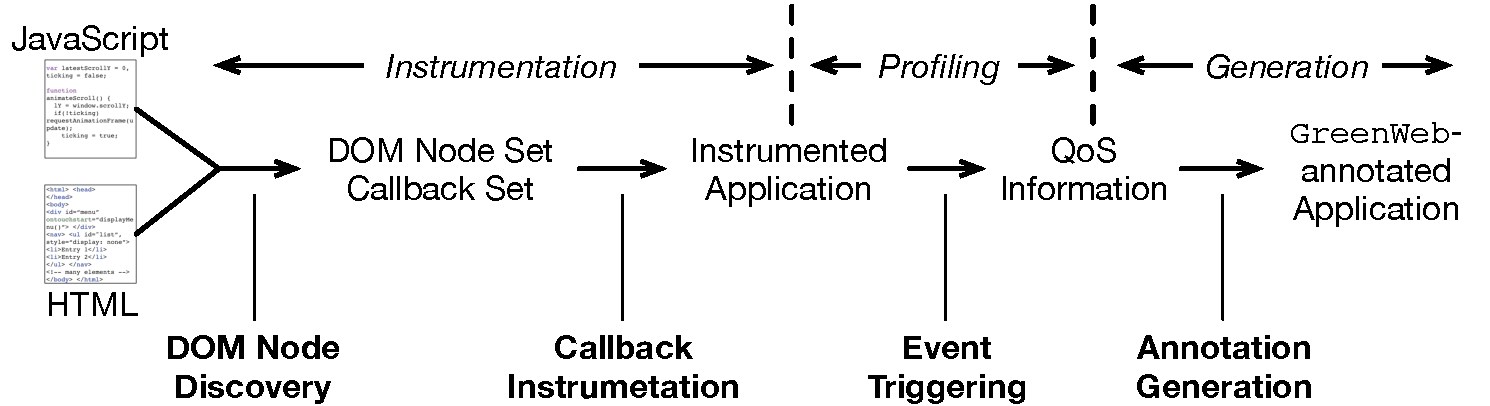
\includegraphics[trim=0 0 0 0, clip, width=\columnwidth]{autogreen}
  \caption{\autogreen's workflow to automatically annotate mobile Web applications with \greenweb APIs.}
  \label{fig:autogreen}
\end{figure}

\autogreen uses the default QoS target values listed in~\Tbl{tab:qos_info} for each detected QoS type. Particularly, for events with a ``single'' QoS type, \autogreen always assumes a short duration. This is because \autogreen does not understand the semantics of an event callback function and has to make conservative decisions about the QoS target information in favor of satisfying QoS over conserving energy.

\section{GreenWeb and WebRT Inteplay}
\label{sec:lang:inter}

\greenweb and \webrt are independent. On one hand, \greenweb does not make any specific assumptions about how the underlying runtime is implemented as long as the runtime is able to make trade-offs between performance and energy consumption. For example, it is possible to use the ACMP-based \webrt as a \greenweb runtime implementation to make QoS-energy trade-offs at the hardware level. It is also feasible to build a runtime leveraging only a single big (or little) core capable of DVFS~\cite{pgdvfs,vsmp}. In addition, one could implement a \greenweb runtime using pure software-level techniques, such as prioritizing resource loading~\cite{klotski} or using power-conserving colors~\cite{chameleon}. 

On the other hand, \webrt does not assume how the QoS requirements is provided to be able to perform scheduling. If not annotated using \greenweb APIs, the QoS information could be defaulted to values that a particular implementation assumes. That is, the \webrt schedulers can assume a default QoS target and QoS type for each Loading, Touching, and Moving interaction. Moreover, the \webrt schedulers could also attempt to infer the QoS type and QoS target by profiling event executions to identify which category in \Tbl{tab:qos_info} that an event falls into.

%Therefore, combining in an integrated system provides programmers an opportunity to guide runtime energy-efficiency optimizations by providing QoS ``hints.''
%I leave the quantitative comparison between unguided and \greenweb-guided \webrt to future work.

\section{Evaluation}
\label{sec:lang:eval}

We evaluate \greenweb in three different aspects. First, we evaluate the \textit{necessity} of \greenweb APIs (\Sect{sec:lang:eval:need}). That is, can a Web runtime automatically infer events' QoS information without developers explicitly providing hints? Second, we evaluate the ``effectiveness'' of the \greenweb APIs (\Sect{sec:lang:eval:effect}). That is, given the annotated QoS information, can a Web runtime effectively optimizes for energy-efficiency while meeting the QoS expectations? Finally, we evaluate the annotation effort in apply \greenweb APIs to Web application (\Sect{sec:lang:eval:annotate}). That is, is the annotation effort lightweight enough to incentive developers to use \greenweb APIs?

To evaluate \greenweb we implement a \webrt-based \greenweb runtime--although note that \webrt and \greenweb are independent as discussed in \Sect{sec:lang:inter}. In particular, the \webrt implementation is exactly the same as what we described in \Sect{sec:runtime}, i.e., based on the ACMP architecture. The software and hardware platform we use the evaluate \greenweb is the same as described in \Sect{sec:runtime:exp}. In addition, we base our evaluation on the same set of applications that are used in evaluating \ebs in \Sect{sec:runtime:ebs:eval}. The details of each application in shown in \Tbl{tab:app}

% !TEX root = ../../paper.tex

\begin{table}[p]
\large
\centering
\captionsetup{width=1\columnwidth}
\caption{Applications used for evaluating \greenweb. They are the same as the ones used for evaluating \ebs in \Sect{sec:runtime:ebs:eval}. ``Annotation'' indicates percentage of events that are annotated. ``Events'' indicates the amount of events triggered during full interaction. Note: we only annotate and count events that are directly triggered by mobile user interactions as discussed in \Sect{sec:runtime:ltm}. Applications marked with * are manually annotated because they are developed using libraries that \autogreen does not currently support. Their annotation percentage numbers are estimated.}
\renewcommand*{\arraystretch}{1.5}
\renewcommand*{\tabcolsep}{6pt}
\resizebox{1\columnwidth}{!}
{
\begin{tabular}{l | c l l | c c}
\toprule[0.15em]
\bigstrut\textbf{Application}  &  \bigstrut\textbf{Interaction} & \bigstrut\textbf{QoS Type}  & \bigstrut\textbf{QoS Target}  & \bigstrut\textbf{Events} & \bigstrut\textbf{Annotation}         \\
\midrule[0.05em]
\website{BBC}          & Loading   & Single        & (1, 10) s          & 60    &  20\%$^*$  \\
\website{Google}       & Loading   & Single        & (1, 10) s          & 26    & 87.5\%       \\
\website{CamanJS}      & Tapping   & Single        & (1, 10) s          & 24    & 100\%    \\
\website{LZMA-JS}      & Tapping   & Single        & (1, 10) s           & 39    & 100\%    \\
\website{MSN}          & Tapping   & Single        & (100, 300) ms         & 126   & 51.2\%    \\
\website{Todo}         & Tapping   & Single        & (100, 300) ms        & 26    & 38.3\%      \\
\website{Amazon}       & Moving    & Continuous    & (16.6, 33.3) ms      & 101   &   33\%$^*$  \\
\website{Craigslist}   & Moving    & Continuous    & (16.6, 33.3) ms    & 22    & 84.6\%      \\
\website{Paper.js}     & Moving    & Continuous    & (16.6, 33.3) ms    & 560    & 100\%   \\
\website{Cnet}        & Tapping   & Continuous    & (16.6, 33.3) ms       & 60    & 55.3\%   \\
\website{Goo.ne.jp}          & Tapping   & Continuous    & (16.6, 33.3) ms     & 23    & 51.8\%    \\
\website{W3Schools}    & Tapping   & Continuous    & (16.6, 33.3) ms      & 59    & 100\%    \\
\bottomrule[0.15em]
\end{tabular}
}
\label{tab:app}
\end{table}



\subsection{Manual Annotation vs. Runtime Mechanism}
\label{sec:lang:eval:need}

As an alternative to receiving QoS annotations (e.g., using \greenweb APIs) from developers, the Web runtime could try to detect QoS information at runtime without language hints. One implementation is to implement the exact logic of \autogreen within the Web runtime. However, there are three major drawbacks of such a runtime-based approach.

First, implementing the QoS detection at runtime is not scalable. For example, whenever the Web standard introduces a new method of implementing animation (i.e., ``continuous'' QoS type) the browser runtime has to be extended to support it. In contrast, with developers directly specifying the QoS type the runtime can confidently optimize for the ``continuous'' QoS type without having to know how an animation is implemented. Second, a pure runtime strategy cannot precisely detect the QoS target information of an event for exactly the same reason that \autogreen cannot precisely detect QoS target. Third, detecting QoS at runtime also introduces runtime performance and energy overhead that could potentially offset the energy saving benefits.

\subsection{Energy-Efficiency Improvement}
\label{sec:lang:eval:effect}

\begin{figure}[p]
\centering
\subfloat[Energy consumption normalized to \textit{Perf}. Lower is better.]
{
        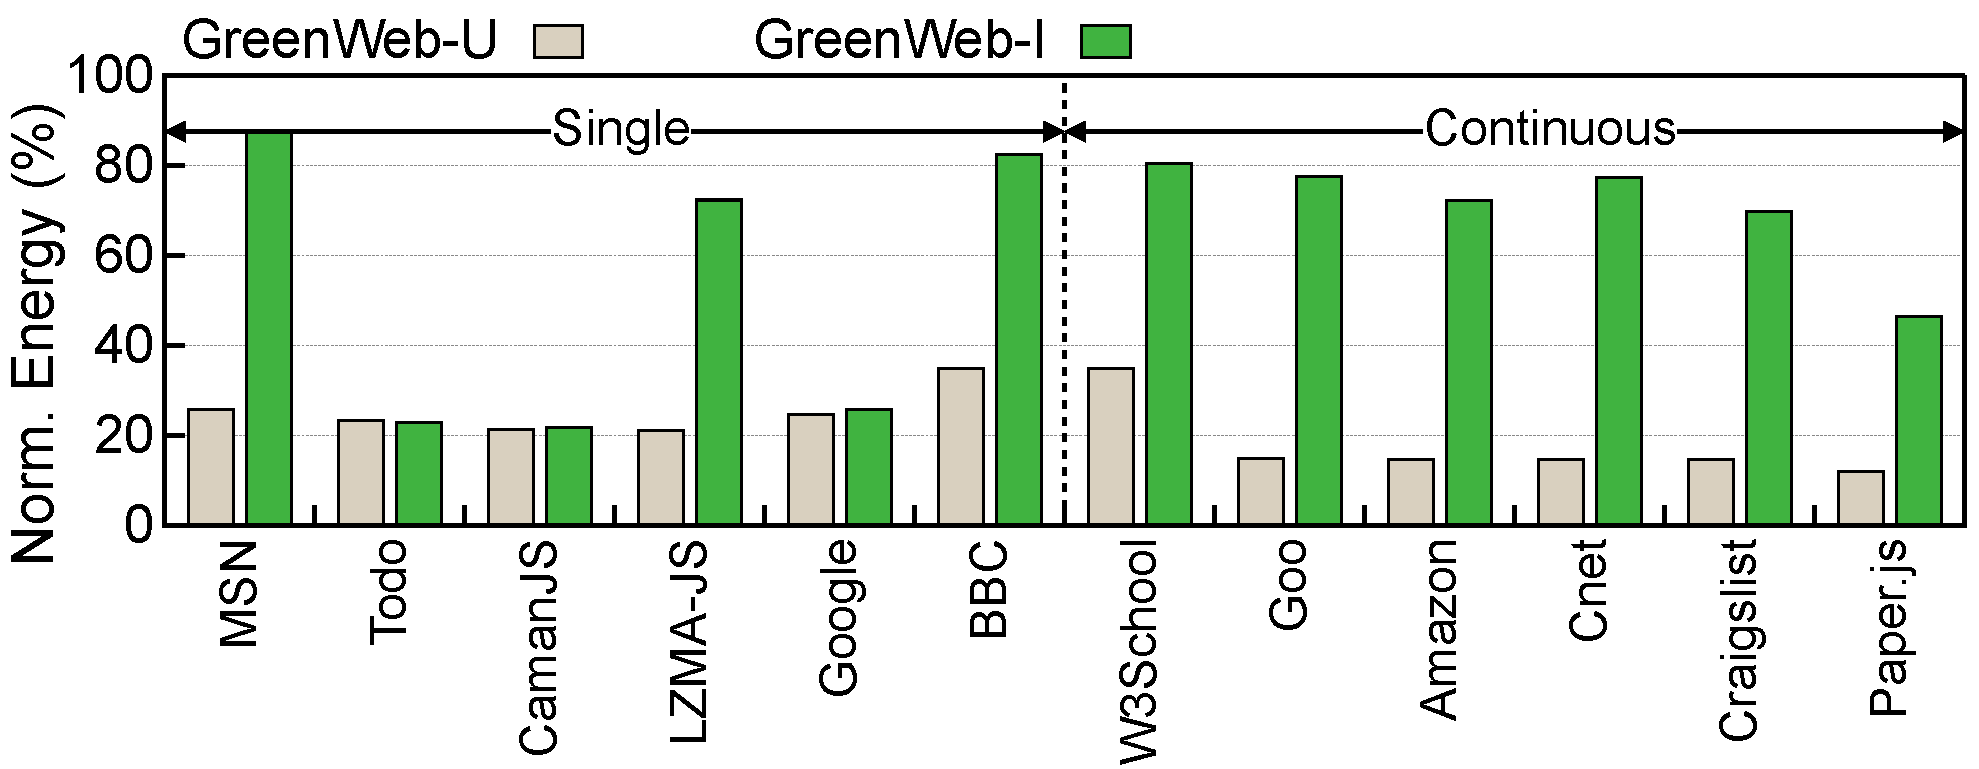
\includegraphics[trim=0 0 0 0, clip, width=1\columnwidth]{energy_results_u}
        \label{fig:energy_results_u}
}\\
\vspace*{25pt}
\subfloat[QoS violations normalized to \textit{Perf}. Lower is better.]
{
        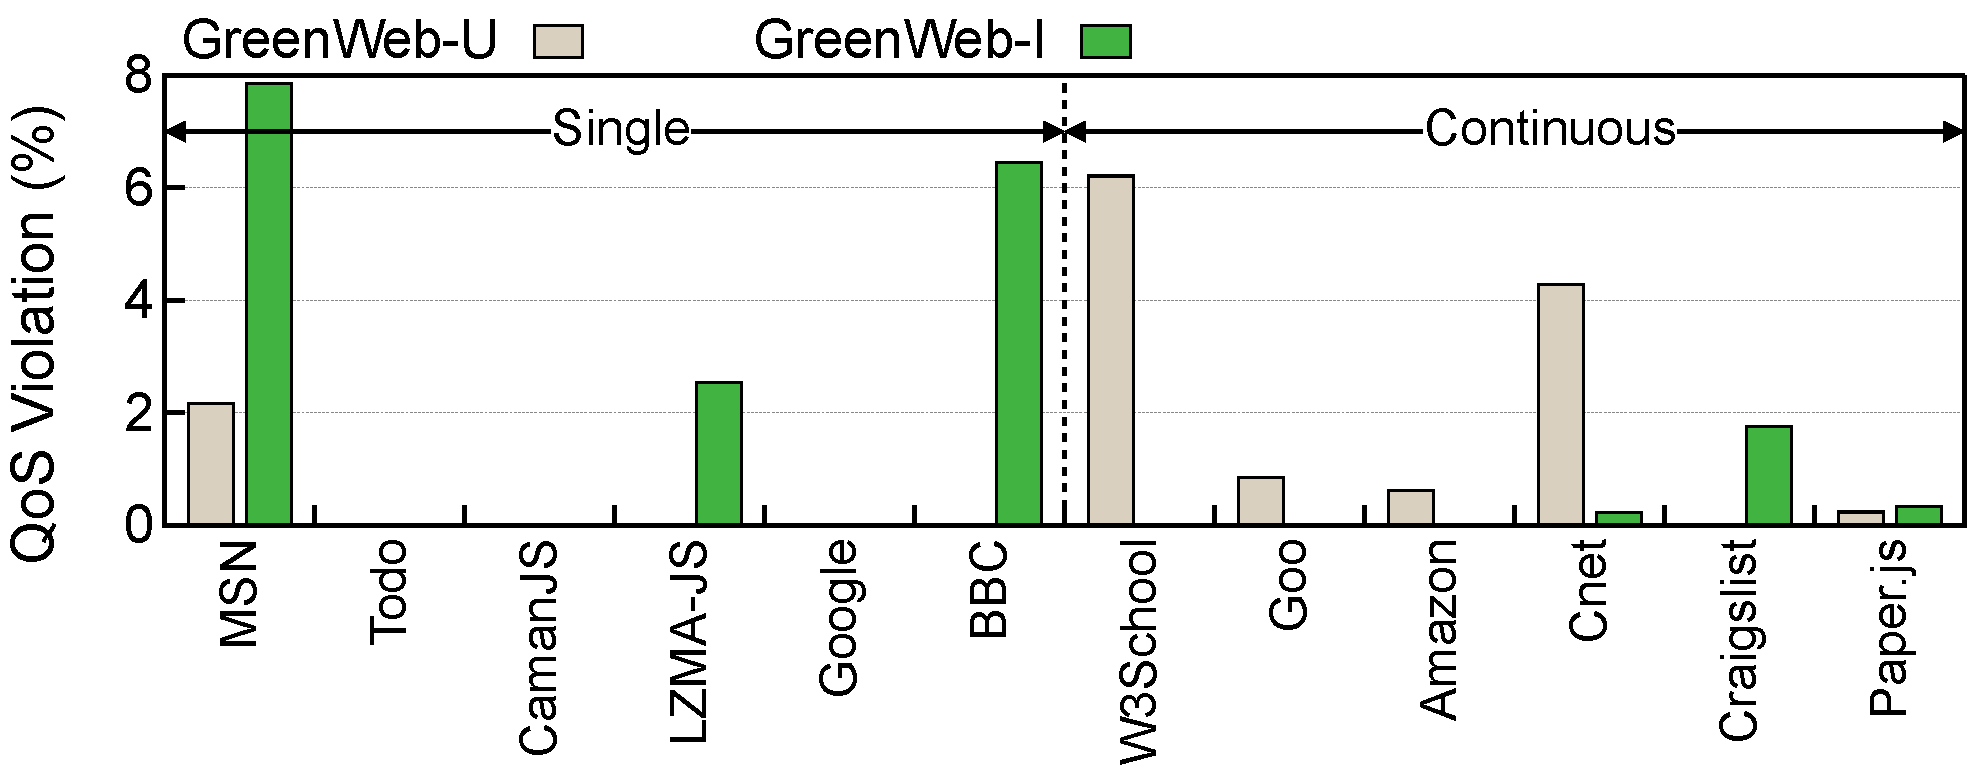
\includegraphics[trim=0 0 0 0, clip, width=1\columnwidth]{qos_results_u}
        \label{fig:qos_results_u}
}
\caption{Microbenchmarking results. Energy numbers are normalized to \textit{Perf}, which provides the best QoS and consumes the most energy. QoS violations are presented as additional violations on top of \textit{Perf}. \textit{GreenWeb-I} and \textit{GreenWeb-U} are \greenweb under two usage scenarios.}
\label{fig:ubenchmark_results}
\end{figure}

To understand the effectiveness of \greenweb on \textit{individual} events, we design a set of microbenchmarking experiments. The goal is to exercise \greenweb on various events that differ in interaction types (LTM), QoS type, and QoS target. To better understand the behavior of \greenweb during microbenchmarking, we compare it only against \textit{Perf}, which always has the highest energy and lowest QoS violation.
%We leave evaluating full interaction of each application to the next subsection.

We construct the microbenchmark set by pairing each application in \Tbl{tab:app} with one of the three primitive interactions (Loading, Tapping, Moving). For each interaction, we manually apply \greenweb annotations. The QoS type and QoS target are determined by the authors visually observing the effect of each interaction. The ``Micro-benchmarking'' category in \Tbl{tab:app} shows details about each microbenchmark. Half of the interactions have a QoS type of ``single'', and the other half have a QoS type of ``continuous.'' Overall, our microbenchmarks cover user events that have different combinations of interaction types, QoS types and QoS targets. 

\paragraph{Energy Savings} \Fig{fig:energy_results_u} shows the energy consumption of \greenweb under both the imperceptible (\textit{GreenWeb-I}) and the usable (\textit{GreenWeb-U}) usage scenarios. The results are normalized to \textit{Perf}. For the diverse set of interactions in our microbenchmark, \greenweb achieves an average 31.9\% and 78.0\% energy saving under the two usage scenarios, respectively. Overall, the energy savings under the usable mode are higher than in the imperceptible mode because the usable QoS target is lower, which allows \greenweb to leverage low energy ACMP configurations more often.

The greatest energy savings in the imperceptible mode come from events in the application \textsf{Todo}, \textsf{CamanJS}, and \textsf{LZMA-JS}. All three events have a ``single'' QoS type, but with different QoS targets (100~ms and 1~s). The frame complexity of the three events is low relative to their QoS target such that \greenweb can meet the QoS target using only little core configurations. \textit{Perf} wastes energy by constantly using the big core with peak frequency. This suggests that \greenweb can adapt to events with different QoS targets.

For all events whose QoS type is ``continuous,'' we see a large difference in energy savings between the imperceptible and usable scenarios. This suggests that in general \greenweb must spend a substantial amount of time on the big core in order to meet the imperceptible QoS target (16.6~ms), but it can use little core configurations most of the time to meet the usable QoS target (33.3~ms). 

\paragraph{QoS Violation} QoS violation is defined as the percentage by which a frame latency exceeds the QoS target. For example, a frame latency of 200~ms leads to an 100\% QoS violation under a 100~ms QoS target. For events with a ``continuous'' QoS type, we report the geometric mean of all associated frames. It is worth noting that although \textit{Perf} behaves the same under the two usage scenarios, its QoS violations are different because the QoS targets are different.

\Fig{fig:qos_results_u} shows the QoS violation of \greenweb on top of \textit{Perf}. On average, \greenweb introduces 1.3\% and 1.2\% more QoS violations than \textit{Perf} under the imperceptible and usable usage scenario, respectively. In the imperceptible mode, three application events (\textsf{MSN}, \textsf{LZMA-JS} and \textsf{BBC}) whose QoS type is ``single'' have relatively high QoS violations. The high QoS violation is primarily introduced by \greenweb's profiling runs to construct the predictive models (see \Sect{sec:runtime:pred}). For example, \textsf{MSN}'s interaction requires peak performance to minimize QoS violations. \greenweb takes two profiling runs, one of which is using the minimum frequency, to adapt to the peak performance. The minimal frequency run causes significant QoS violations. In contrast, events that have a ``continuous'' QoS type trigger a large amount of frames. Therefore, the profiling overhead is effectively amortized, and their QoS violations are negligible.

Some events that have a ``continuous'' QoS type have relatively high QoS violations under the usable mode. Outstanding examples are \textsf{W3School} and \textsf{Cnet}. Our analysis shows that most of the QoS violations come from frame complexity surges in a continuous frame sequence. \greenweb aggressively scales down performance when the QoS target is low, and did not always react to the sudden frame complexity increase quickly. This suggests that the \greenweb runtime could be better enhanced to capture the pattern of frame fluctuation in an event, potentially through offline profiling~\cite{pgdvfs}.

\subsection{Annotation Effort}
\label{sec:lang:eval:annotate}

It is important to keep the annotation process lightweight  because a \greenweb-based system requires Web applications to be explicitly annotated. Manually annotating the QoS information of each event is time consuming for two reasons. First, real Web applications typically contain tens or even hundreds of events, as shown in \Tbl{tab:app}. Second, one would have to understand the event callback semantics to determine the QoS type and QoS target of each event, which makes it difficult to annotate unfamiliar code, which in turn makes \greenweb impractical to use in real Web development.

Through our experience with evaluating \greenweb on real Web applications, we find that the best practice is to use a combination of \autogreen and manual annotation. We use \autogreen because it greatly improves productivity. Throughout all benchmarked applications, \autogreen finishes annotations under 1 minute for an entire annotation.

The downside of \autogreen is that it does not always annotate QoS targets correctly because it conservatively assumes short response latency for events with a ``single'' QoS type (see discussion in \Sect{sec:lang:auto}). Therefore, we manually correct the QoS target for events that should have a long response latency. Overall, we find that the percentage of events whose QoS type is ``single'' is below 20\% for all applications. Most application events have a QoS type of ``continuous'', corroborating the prevalence of animation in today's Web applications. The ``Annotation'' column in \Tbl{tab:app} shows that in the end we annotate over 50\% of all events in most applications. Unannotated events are not directly triggered by mobile user interactions and therefore are not the optimization target of \greenweb, as discussed in~\Sect{sec:runtime:ltm}.

Overall, it took us about 5 $\sim$10 minutes to annotate each application with the combined manual and automatic approach. While we are not familiar with each application's codebase, the annotation is not a labor-intensive process. We expect the overhead to be even lower for experienced developers who are more familiar with their own applications.

\section{Discussion}
\label{sec:lang:disc}

\paragraph{Effectiveness in a Multi-application Environment} The ACMP-based \greenweb runtime implementation presented here assumes that all CPU resources in a SoC are available to the foreground Web application during scheduling. We believe that this ACMP-based runtime design is also applicable when multiple mobile applications are concurrently consuming CPU resources. The reason is two-fold.

First, today's ACMP systems have ample CPU resources, e.g., four big and four small cores in the Exynos 5410 SoC with each core cluster having DVFS capability. If there is a background application occupying some CPU resources, the \greenweb runtime system will still have a large trade-off space to schedule, although with fewer resources. Second, today's mobile SoCs are on the verge of supporting fine-grained power management techniques such as per-core DVFS using integrated voltage regulators (IVRs)~\cite{ivr}. Therefore, the scheduling space will become larger to further accommodate concurrent applications in the near future.

\paragraph{Defense Against Mis-annotation} One potential vulnerability of exposing \greenweb hints to developers is that developers might place hints that lead to inefficient system decisions. For example, a developer could set every event's QoS target to an extremely low value, which causes the Web runtime always to operate at the highest performance with maximal energy consumption. Such a mis-annotation could be introduced either inadvertently as a program energy bug or intentionally as an adversarial attack.

The notion of user-agent intervention (UAI)~\cite{useragentintervention} in the Web community can be used to defend against such an issue. In short, UAI contends that a Web platform should correct application behaviors that are deemed harmful or undesired. Most of today's Web runtime systems have already implemented plenty of UAI policies such as blocking malicious third-party scripts or re-prioritizing resource loading order under latency/bandwidth constraints. Similarly, a Web runtime could adopt a \greenweb-specific UAI policy. One candidate is to specify an energy budget of any Web application and ignores overly aggressive \greenweb annotations once the energy budget is consumed. We leave it as future work to define, express, and implement such a UAI policy.

\paragraph{Composability of QoS Abstractions} Although the QoS type and QoS target abstractions are sufficient for expressing predominant QoS specifications on \textit{today}'s mobile devices, in the long term we will see new user interaction forms (e.g., using visible light~\cite{license}) and new ways that users assess QoS experience. Therefore, it is important to design ``primitive'' QoS abstractions, based on which complex, higher-level QoS abstractions can be easily composed.

The composability of QoS abstractions is critical because enumerating every single possible kind of QoS experience in a Web programming model is not scalable. Instead, the Web programming model should ideally provide a QoS primitive library that lets developers construct different QoS specifications in a completely customized way. To achieve this goal will likely involve extensively surveying future human-computer interaction forms and new QoS specifications. We leave it for the next phase of research.

\section{Related Work}
\label{sec:lang:related}

We first discuss \greenweb in the context of prior work on language support for Web performance (\Sect{sec:lang:related:perf}). Although there exists little prior work on language support for Web energy-efficiency, language extensions for general energy optimizations do exist, which we compare and contrast \greenweb against in (\Sect{sec:lang:related:energy}). Finally, we discuss why the two QoS abstractions we propose are more comprehensive than prior work on mobile QoS characterizations (\Sect{sec:lang:related:qos}).

\subsection{Language Support for Web Performance}
\label{sec:lang:related:perf}

The Web community has a long tradition of providing language extensions that allow developers to specify ``hints'' for browsers. The focus, however, has been primarily on \textit{performance} optimizations. \greenweb, to the best of our knowledge, is the first Web language extension that specifically targets \textit{energy}.

The most classical example of performance hint is link prefetch~\cite{linkprefetch}, which lets Web developers use an HTML tag to specify that a particular link will likely be fetched in the near future. With such information, a Web browser could prefetch the link when there are no on-demand network requests. Another example is the CSS \texttt{willChange} property~\cite{csswillchange}, which hints browsers about what visual changes to expect from an element so that the browser could perform a computationally intensive task ahead of time. Similar to \texttt{willChange}, \greenweb introduces a new CSS property \texttt{onevent-qos}, which allows providing QoS-related hints.

\subsection{Language Support for Energy Efficiency}
\label{sec:lang:related:energy}

Language support for energy efficiency has recently become a major research thrust. Most work targets sensor-based applications and approximate computing whereas \greenweb, to the best of our knowledge, is the first to focus on Web applications. In addition, most previously proposed language systems require developers to annotate applications manually. We show that \greenweb annotations can be automatically applied without programmer intervention. We now compare \greenweb with prior language proposals in greater detail.

Eon~\cite{eon} provides language constructs that let developers express alternative program control flow paths and associate energy states with control flows, based on which the runtime selects control flow paths that are suitable given the device energy level. Green~\cite{green} provides APIs that let developers specify multiple approximate versions of a function and QoS loss constraints, which guide the runtime to save energy without violating QoS. Both proposals rely on developers supplying alternative implementations, which is an optimization not immediately applicable to Web applications. In the future, however, it would be interesting to evaluate such an optimization strategy in the Web domain.

Energy Types~\cite{energytypes} and EnerJ~\cite{enerJ} take the language support for energy-efficiency a step further by designing general type systems. Both work ensures sound and safe energy optimizations by enforcing static type checking. Both type systems target imperative programming, and therefore are not immediately applicable to Web programming which is inherently declarative. In the future, however, it would be interesting to study how to decorate DOM elements with different type qualifiers to guide the energy optimizations.

LAB~\cite{lab} identifies latency, accuracy, and battery as fundamental abstractions for improving energy efficiency in sensor-based applications. Similarly, \greenweb identifies the QoS type and QoS target abstractions for enabling energy-efficient Web applications.

\subsection{Mobile QoS Characterization}
\label{sec:lang:related:qos}

The two QoS abstractions and the design of \greenweb APIs is driven by understanding application QoS requirements from an application events perspective, which is not the focus in the majority of existing mobile workload suite and benchmark~\cite{jsbench,BrowsingBench,BrowserMark,MobileBench,Moby,Vellamo,AnTuTu,sunspider,Octane,Kraken,GeekBench}. Other benchmarks consider only a particular form of QoS. For example, BBench~\cite{BBench} considers the webpage load time as the QoS constraint for Web browsing; the Web latency benchmark~\cite{WebLatencyBenchmark} considers the event latency of user actions to webpage elements; the GFXBench~\cite{GFXBench} and BaseMark~\cite{BaseMark} benchmarks consider FPS. However, our QoS abstractions lead to a general methodology to identify QoS requirements of a wide range of applications.
